\section{Generalized Critic Policy Optimization}
\label{sec:method}

Let us consider the case of a msjmdq. The set of actions $\mathcal{A}$ and the set of states $\mathcal{S}$ are continuous. $\pi$ is a gaussian probability distribution.

We present the following model for Actor-Critic methods:

GC(V,)
Let $\mathcal{F}: \mathbb{R}^n \mapsto \mathbb{R}$ be the aggregate function


%Test the method with different algorithms
%they need to be actor-critic algorithms
%will our method be implemented differently to include each algorithm's tricks? or will we only implement it on top of algorithms that do not require modifications?

%tableaux : lignes: algorithmes2baz, algorithmes + amélioration, algorithmes + améliorations d'autres articles. colonnes : tasks

%\begin{tabular}
%\end{tabular}
fsd $\pi$ is a continuous probability distribution
\begin{figure}[!htb]
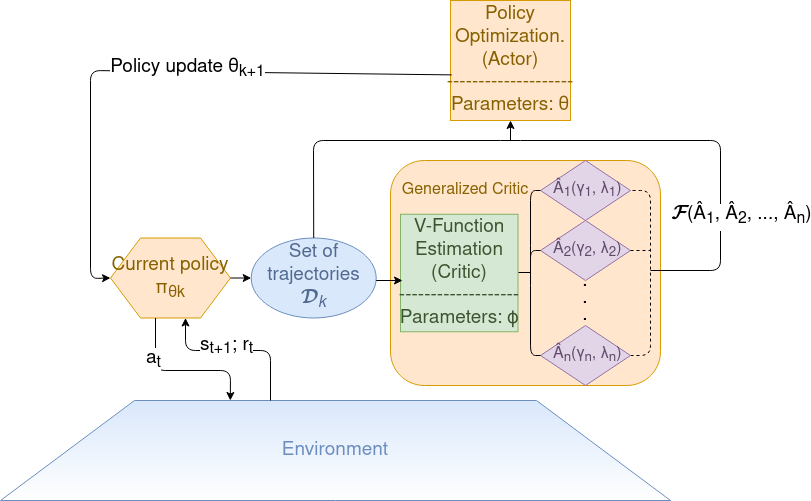
\includegraphics[width=8.5cm]{images/model}
\caption{Multi-advantage critic}
\label{fig:model}
\end{figure}

% Speak about function F(A1, A2, ...) 
%

